\subsection{Problem Formulation}
Consider $N$ native  proteins configurations $P_{i}^{nat}$, $i=1...N$.
For each protein complex number $i$ we generate $D$ decoys, $P_{ij}^{nonnat},$ $j=1...D$, where the first index runs over different protein 
complexes and the second index runs over decoys. 
Our goal is to find  a \emph{scoring functional} $F$, defined for all 
possible protein-protein complex
structures (the set $\mathbb{P}$), such that for each native complex $i$ and its nonnative decoy $j$ the following inequality holds: 
\begin{eqnarray}
\label{eq:complexes}
F(P_{i}^{nat}) < F(P_{ij}^{nonnat}) 
\end{eqnarray}
%:
There are many ways to construct the functional $F$ (Eq. \ref{eq:complexes}). To outline its form, we are relying on the following assumptions:
\begin{enumerate}
\item Functional $F$ depends only on the interface between the proteins. We define the interface as a set of all atom pairs at a distance smaller 
than a certain cutoff distance  
$r_{max}$, such that the first atom in each pair belongs to the first protein and the second atom in each pair belongs to the second protein.

\item The protein is represented as a set of discrete interaction sites that are located at the centers of the atomic nuclei. All interaction sites are divided into $M$ types according to the properties of the corresponding atomic nuclei.
In this study we choose $M=20$.

\item Functional $F$ depends only on the distribution of the distances between the interaction sites (the number of site pairs at a certain distance),
%
\begin{equation}
F(P)=F(n^{11}(r),..,n^{kl}(r),..,n^{mm}(r)) = F(n(r))
,
\end{equation}
where $n^{kl}(r)$ is the \emph{number density of site-site pairs} separated by a distance $r$, with site $k$ located on the first protein, 
and site $l$ located on the second protein. For homogeneous systems, such as liquids,  functions $n^{kl}(r)$ can be expressed via 
site-site radial distribution functions $g^{kl}(r)$, which can be obtained experimentally, as $n^{kl}(r)=4\pi r^2 \rho g^{kl}(r) N_a$, where 
$\rho$ is the number density and $N_a$ is the total number of atoms in the system \cite{Hansen2006}. 
However, for proteins this is not the case. 

\item $F$ is a linear functional, $F(\alpha n_1(r) +\beta n_2(r)) = \alpha F( n_1(r)) +\beta F( n_2(r))$.
\end{enumerate}

One of the simplest functionals $F(n(r))$ fulfilling these assumptions can be written as:
\begin{eqnarray}
\label{eq:functional}
F(n(r))\equiv F(n^{11}(r),..,n^{kl}(r),..,n^{MM}(r)) = \sum_{k=1}^M \sum_{l=k}^M \int \limits_{0}^{r_{max}} n^{kl}(r)U^{kl}(r)~dr 
\end{eqnarray}
It contains unknown functions $U^{kl}(r)$ that can be determined from the training set of native protein complexes. 
From now on,  we will call these  functions \emph{scoring potentials}.\footnote{Though the scoring function (Eq. \ref{eq:functional}) is 
similar by the structure to e.g. the excess internal energy \cite{Hansen2006}, our scoring potentials $U^{kl}(r)$ are not equal to the 
potential energy functions between sites $k$ and $l$.} Once the scoring functions are known, to compute the value of $F$ we need to 
specify site-site number densities $n^{kl}(r)$. In practice, we calculate them as a sum of all $k-l$ distances in a given protein complex using the 
equation:
\begin{eqnarray}
n^{kl}(r) = \sum_{ij} \frac{1}{\sqrt{2\pi \sigma^2}} e^{-{\frac{(r-r_{ij})^2}{2\sigma^2}}}
,
\label{eq:number_density}
\end{eqnarray}
where each distance distribution is represented with a Gaussian  centered at $r_{ij}$ with the variance of $ \sigma ^ 2 $. 
The sum is taken over all $k-l$ site pairs $i$ and $j$ separated by the distance $r_{ij}$ smaller than $r_{max}$, with site $k$ located 
on the first protein of the complex, and site $l$ located on the second protein. In the limiting case of the variance tending to zero, 
Eq. \ref{eq:number_density} turns into a sum over Dirac delta functions. In our study we assume the value of $ \sigma $ to be fixed
for all site-site distributions. However, if one has an additional information about individual distance distributions, e.g. Debye-Waller factors,
 molecular dynamics trajectories, etc., it can be used for more precise parametrization of the variance or even instead of the Gaussian approximation
 in Eq. \ref{eq:number_density}. Finally, we compute the score of each conformation using equation 
\footnote{ Generally, 
if the distance distributions have a non-Gaussian shape, $n^{kl}(r) = \sum_{ij} f(r-r_{ij})$, functions $ \Upsilon^{kl}(r)$ will be computed as a 
convolution  $\Upsilon^{kl} =  f \ast U^{kl}$.}:

\begin{eqnarray}
\label{eq:scoring_1}
\mathrm{Score} =  \sum_{ij}  \Upsilon^{kl}(r_{ij}) 
\end{eqnarray}
where the sum is taken over all pairs of atoms $i$ and $j$ separated by the distance $r_{ij}$ 
smaller then $r_{max}$, with atom $i$ of type $k$ located on the first protein of the complex, and atom $j$ 
of type $l$ located on the second protein. The function $ \Upsilon^{kl}(r)$ is the Gauss transform of the scoring potential $U^{kl}(x)$:

\begin{eqnarray}
\label{eq:scoring_2}
 \Upsilon^{kl}(r) =\frac{1}{\sqrt{2\pi \sigma^2}}  \int \limits_{0}^{r_{max}} e^{-{\frac{(x-r)^2}{2\sigma^2}}} U^{kl}(x)~dx
\end{eqnarray}
%=======================================================================================================%

\subsection{Expansion of $U(r)$ and $n(r)$ in an orthogonal basis}
Given a set of functions $\xi_p (r)$ orthogonal on the interval $[r_1;r_2]$ with a nonnegative weight function $\Omega(r)$ such that
\begin{eqnarray}
\int \limits_{r_1}^{r_2} \xi_{p_1}(r) \xi_{p_2}(r) \Omega(r)~dr = \delta_{p_1 p_2}
\label{eq:orth}
,
\end{eqnarray}
where $\delta_{p_1 p_2}$ is the Kronecker delta function, scoring potentials $U_{kl}(r)$ and number densities $n_{kl}(r)$ can be expanded on the interval $[r_1;r_2]$ as:

\begin{eqnarray}
\label{eq:expU}
U_{kl}(r)=\sum_p w_p^{kl} \xi_p (r) \sqrt{ \Omega(r)},~~~~r \in [r_1;r_2] \\
n_{kl}(r)=\sum_p x_p^{kl} \xi_p (r) \sqrt{ \Omega(r)},~~~~r \in [r_1;r_2]
\label{eq:expg}
\end{eqnarray}

Expansion coefficients $w_p^{kl}$ and $x_p^{kl}$ can be determined from the orthogonality condition (Eq. \ref{eq:orth}) as 
\begin{eqnarray}
w_p^{kl} = \int \limits_{r_1}^{r_2}U_{kl}(r) \xi_p (r) \sqrt{ \Omega(r)}~dr \\
x_p^{kl} = \int \limits_{r_1}^{r_2}n_{kl}(r) \xi_p (r) \sqrt{ \Omega(r)}~dr
\label{eq:projection}
\end{eqnarray}

Using expansions Eq. \ref{eq:expU} and Eq. \ref{eq:expg}, the functional $F(n(r))$ can be rewritten as:

\begin{eqnarray}
F(n(r))= \sum_{k,l}^M\int \limits_{0}^{r_{max}}  \sum_{p_1}\sum_{p_2}w_{p_1}^{kl}x_{p_2}^{kl}\xi_{p_1}(r)\xi_{p_2}(r) \Omega(r) ~dr
\end{eqnarray}

In this study we use two types of functions $\xi_p (r)$ orthogonal on the interval $[0;10]$  with a unit weight, 
(i) shifted Legendre polynomials and (ii) traditionally used shifted rectangular functions. These two types of functions are plotted in Fig. 
\ref{fig_Basis}. Other types of orthogonal functions can also be used. 
If the functions $\xi_p (r)$ are chosen to be negligibly small outside the interval $[0;r_{max}]$ or if their interval of orthogonality $[r_1;r_2]$ 
coincides with the interval $[0;r_{max}]$, as is the case for two sets of our functions, then the scoring functional $F(n(r))$ can be expanded up 
to the order $P$ as:

\begin{eqnarray}
\label{eq:expansion}
F(n(r)) \approx \sum_{k=1}^M\sum_{l=k}^M \sum_{p}^{P} w_{p}^{kl}x_{p}^{kl} = (\mathbf{w} \cdot \mathbf{x}),~~~~\mathbf{w}, \mathbf{x} \in \mathbb{R}^{P \times M \times (M+1)/2}
\end{eqnarray}
We will refer to the vector $\mathbf{w}$ as to the \emph{scoring vector} and to the vector $\mathbf{x}$  as to the  \emph{structure vector}.
Equations \ref{eq:number_density} and \ref{eq:projection} provide the projection from a protein complex  structure into the \emph{scoring space}  $\mathbb{R}^{P \times M \times (M+1)/2}$. 
Using these formulas, we can project structural information of each protein complex into a certain structure vector $ \mathbf{x}$ on  $\mathbb{R}^{P \times M \times (M+1)/2}$. 

\begin{figure}[H]
\begin{center}
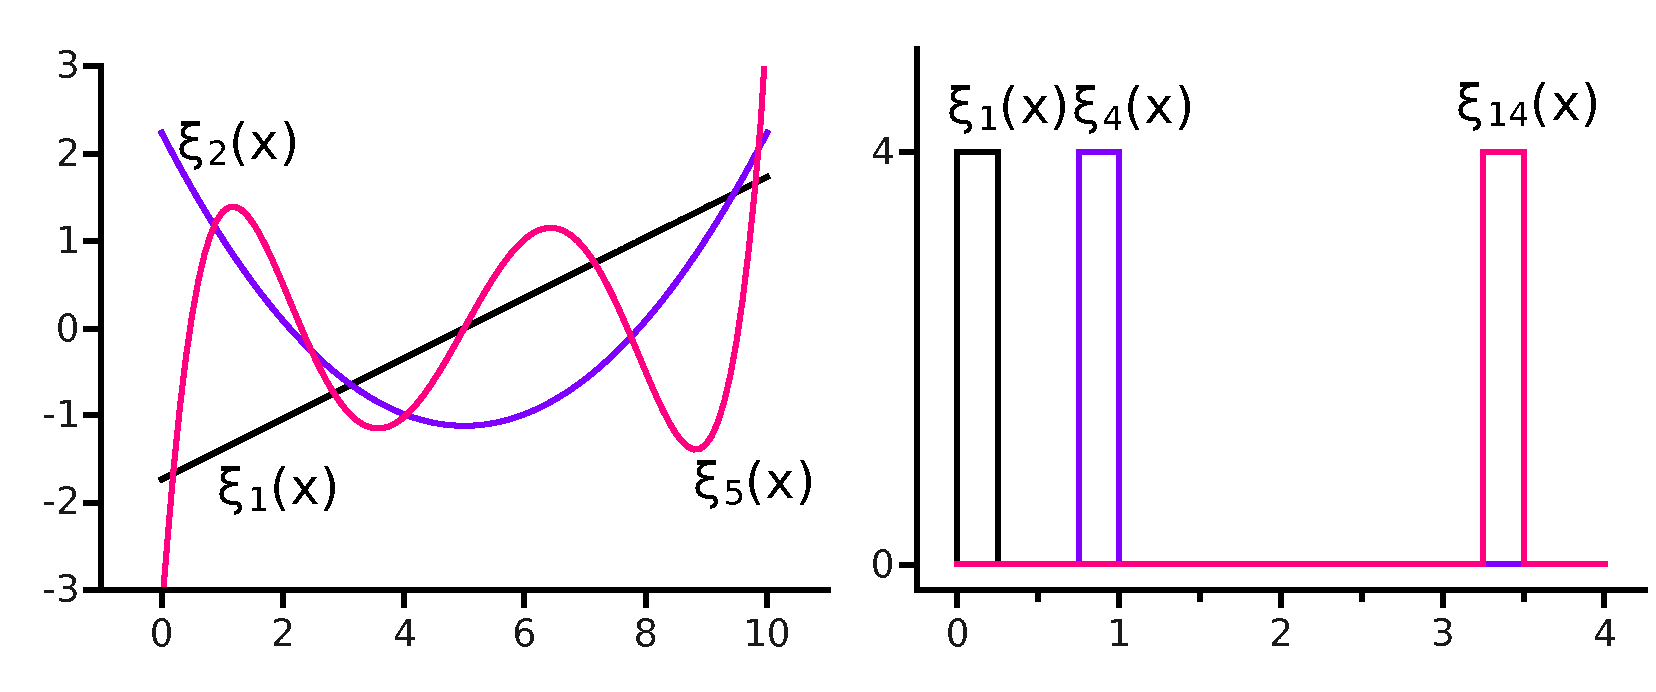
\includegraphics[scale=0.5]{Scoring/Fig/Basis_01.pdf}
\caption[Two types of orthogonal functions]{Two types of orthogonal functions. 
Left: shifted Legendre polynomials orthogonal on the interval $[0;10]$.
Right: shifted rectangular functions.
}
\label{fig_Basis} 
\end{center}
\end{figure}



%=======================================================================================================%

\subsection{Geometrical interpretation and connection to quadratic programming}
Using the expansion of the scoring functional $F$ provided by Eq. \ref{eq:expansion}, we can reformulate the scoring problem (Eq. \ref{eq:complexes}) as follows -- 
given $N$ native structure vectors $\mathbf{x}_{i}^{nat}$ and $N \times D$ nonnative structure vectors $\mathbf{x}_{ij}^{nonnat}$, find a scoring 
vector $\mathbf{w} \in  \mathbb{R}^{P \times M \times (M+1)/2}$ such that:
\begin{eqnarray}
\forall i=1...N, \forall j=1...D ~~~(\mathbf{x}_{i}^{nat} \cdot \mathbf{w})<(\mathbf{x}_{ij}^{nonnat} \cdot \mathbf{w}),
\end{eqnarray}
or, equivalently,  
\begin{eqnarray}
\label{eq:planes}
\forall i=1...N, \forall j=1...D ~~~([\mathbf{x}_{ij}^{nonnat}-\mathbf{x}_{i}^{nat}] \cdot \mathbf{w})>0),
\end{eqnarray}
%
which is a set of $N \times D$ \emph{half-space equations} in $\mathbb{R}^{P \times M \times (M+1)/2}$. Each of the half-spaces is 
defined by a plane in   $\mathbb{R}^{P \times M \times (M+1)/2}$ with the common normal $ \mathbf{w}$. Thus, \emph{finding the scoring 
vector is equivalent to finding the common normal $ \mathbf{w}$} to the planes in 
Eq. \ref{eq:planes}.
Geometrical representation of three groups of  structure vectors separated by three parallel hyperplanes with the common normal  $ \mathbf{w}$ is given 
in Fig. \ref{fig:BSVM}.

\begin{figure}[H]
\begin{center}
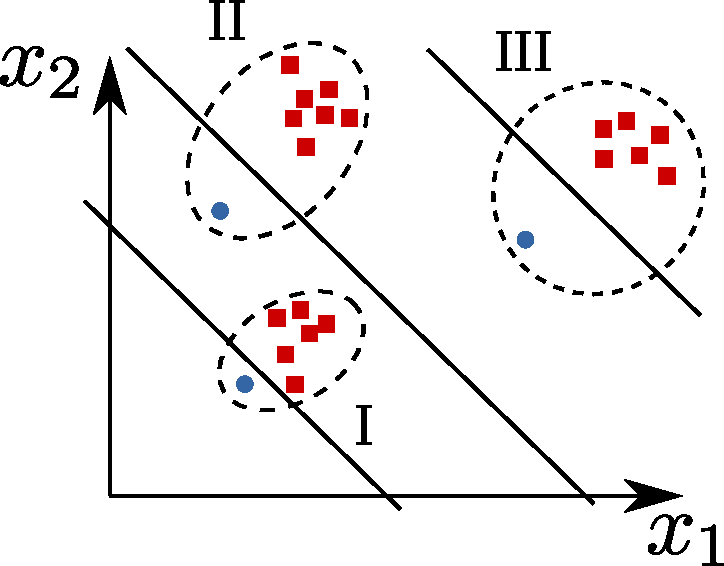
\includegraphics[scale=0.5]{Scoring/Fig/BSVM_single_point.pdf}
\caption[Structure vectors for three complexes]{Structure vectors for three complexes are shown. Native structure vectors are plotted as blue circles. 
Nonnative structure vectors are plotted as red squares. 
Native structure vectors in each complex are separated from nonnative ones by three hyperplanes with a common normal. 
This normal is the scoring vector $\mathbf{w}$ we are aiming to find.
}
\label{fig:BSVM} 
\end{center}
\end{figure}

In the training set, some decoy structures can be very close to the native structures. In practice, we define the native structure as a structure with ligand 
root-mean-square deviation (lRMSD) smaller than 2 \AA. Therefore, for each complex we may have several  native structure vectors along with 
several nonnative structure vectors. Now the question is -- how do we determine the set of separating hyperplanes shown in  Fig. \ref{fig:BSVM} with common 
normal $\mathbf{w}$? To answer this question we first consider two special cases presented below.

\subsubsection{Case I. Existence of many solutions}
In Fig. \ref{fig:MNSolutions}A we present an example of a single complex when infinitely many hyperplanes can separate  
 two classes of structure vectors. 
 A similar example can be easily constructed for the case with multiple complexes. 
 In case of two classes of vectors, Vapnik proposed to use a special kind of separator, the so-called \emph{optimal separating hyperplane} \cite{Vapnik2000}, 
 which is unique and maximizes the distance to the closest point from either class. 
 We can generalize this idea and formulate the following \emph{quadratic 
programming optimization} problem:
 \begin{eqnarray}
 \begin{array}{lcl} 
\mathrm{Minimize ~(in  ~\mathbf{w}, ~b_j)} &  \frac{1}{2} \mathbf{w} \cdot \mathbf{w}\\
\label{eq:svmPrimal1}
\mathrm{Subject~to}& y_{ij} \left[ \mathbf{w} \cdot \mathbf{x}_{ij}-b_j \right]-1 \geq 0, ~ i=1...N,~j=1...D
\end{array}
\end{eqnarray}
where $y_{ij} = -1$ when the structure vector $\mathbf{x}_{ij}$ is native and $y_{ij} = 1$ otherwise.
Now we are ready to formulate
%
\begin{lemma}
If exists such a linear scoring functional of form of Eq. \ref{eq:expansion} that correctly discriminates the native structure vectors for all 
complexes (Eq. \ref{eq:planes}), then the optimal scoring vector is unique and given by the solution of problem (Eq. \ref{eq:svmPrimal1}).
%\label{lemma1}
\end{lemma}
%
\begin{remark}
The scoring vector is optimal in the sense that it maximizes the separation between native and nonnative structure vectors.
\end{remark}
Generally, such a linear scoring functional (with a fixed value of the expansion order $P$) may not exist, as demonstrated below. 
Therefore, we will have to modify the optimization problem (Eq. \ref{eq:svmPrimal1}). 

 \subsubsection{Case II. No solution exists}
   In Fig. \ref{fig:MNSolutions}B we present an example when no hyperplane can separate the two classes of the structure 
vectors of a single 
complex. For this case, Cortes and Vapnik proposed to relax the condition for the optimal separating hyperplane \cite{Cortes1995}, including 
an additional term. This term minimizes the sum of penalties for misclassified vectors. We again generalize this idea and introduce for each 
decoy set $j=1...D$ \emph{slack variables} $\xi_{ij}$, which are positive for misclassified structure vectors and zero otherwise. 
A non-zero value of  $\xi_{ij}$ allows the structure vector $x_{ij}$ to overcome the inequality condition in Eq. \ref{eq:svmPrimal1} at a cost 
proportional to the value of  $\xi_{ij}$ (see Fig. \ref{fig:MNSolutions}B). The new \emph{soft-margin} quadratic optimization problem reads: 

\begin{eqnarray}
\label{eq:svmSoftMargin}
\begin{tabular}{lc}
Minimize (in  $\mathbf{w}$, $b_j$, $\xi_{ij}$):& $\frac{1}{2} \mathbf{w}\cdot\mathbf{w}+ \sum_{ij}C_{ij}\xi_{ij}$ \\ 
\multirow{2}{*}{Subject to:}
&$y_{ij} \left[ \mathbf{w}\cdot \mathbf{x}_{ij}-b_j \right]-1 +\xi_{ij} \geq 0, ~ i=1...N,~j=1...D$ \\
&$\xi_{ij} \geq 0$
\end{tabular}
\end{eqnarray}

The solution of this problem provides a trade-off between how large will be the separation between two classes of the structure vectors of each 
complex and how many misclassified vectors will be in the solution. Parameters $C_{ij}$ can be regarded as {\em regularization parameters}. 
The solution of Eq. \ref{eq:svmSoftMargin} tends to maximize the structure vector separation for small values of $C_{ij}$ or minimize the number 
of misclassified structure vectors for large values of  $C_{ij}$. We choose parameters $C_{ij}$ to be different for native and nonnative structure 
vectors of each complex because fewer native structure vectors should have the larger weight (see for instance \cite{Akbani2004}). 
%
The following lemma provides the foundation for the numerical scheme used in this work:
%
\begin{lemma}
The optimal scoring vector is unique and given by the solution of problem (Eq. \ref{eq:svmSoftMargin}).
\label{lemma2}
\end{lemma}
%
\begin{remark}
Here, the scoring vector is optimal in the sense that it maximizes the separation between native and nonnative structure vectors and minimizes the 
number of misclassified vectors. Regularization parameters $C_{ij}$ in Eq. \ref{eq:svmSoftMargin} tune the importance of either factors.
\end{remark}
%
The proof of lemmas (1, 2) can be found, e.g., in \cite{Crisp2000}.
Overall, the formulation of the optimization problem (Eq. \ref{eq:svmSoftMargin}) is very similar to the formulation of soft-margin 
\emph{support vector machine} (SVM) problem \cite{Cortes1995}. Therefore, to solve this problem (Eq. \ref{eq:svmSoftMargin})
 we will use techniques developed for SVM.
\begin{figure}[H]
\begin{center}
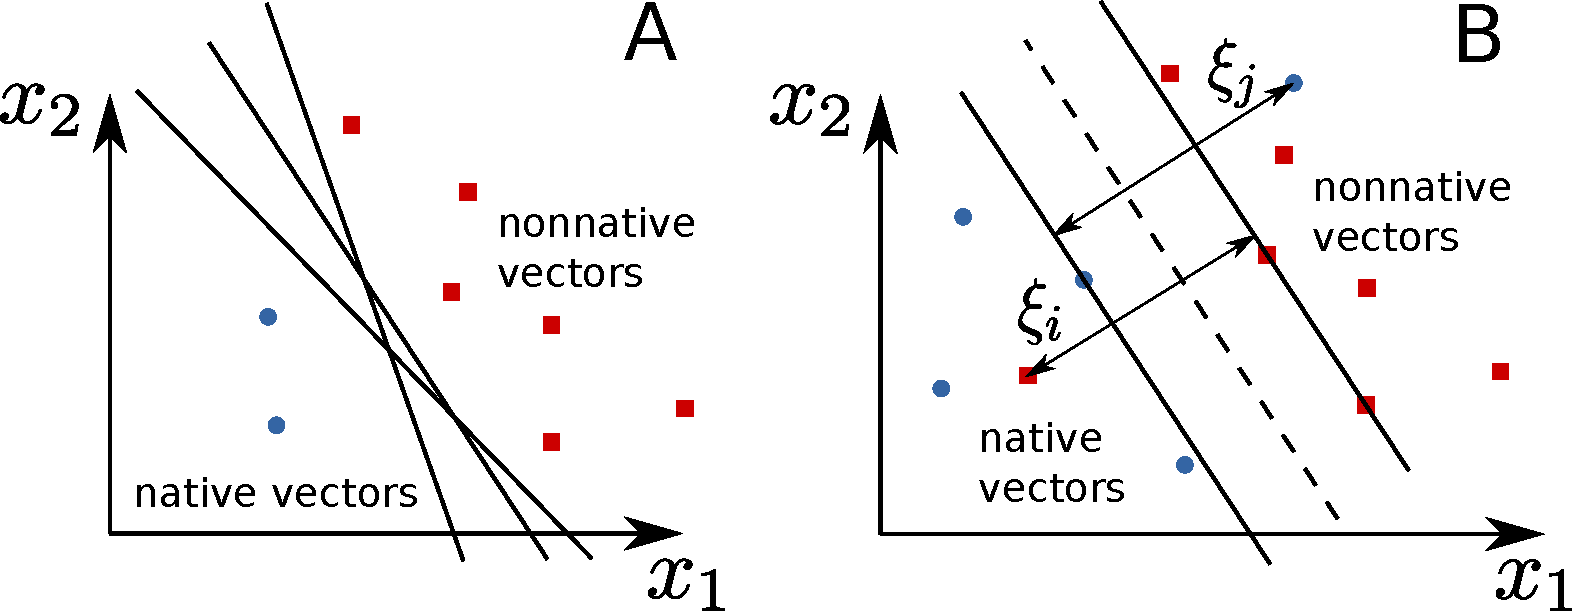
\includegraphics[scale=0.5]{Scoring/Fig/MNSolution_7Sep_1.pdf}
\caption[Two classes of structure vectors for a single complex]{Two classes of structure vectors for a single complex are shown. 
Native structure vectors are plotted as blue circles. 
Nonnative structure vectors are plotted as red squares. 
A) The case when infinitely many hyperplanes can separate the two classes. 
B) The case when no optimal separating hyperplane exists. 
Slack variables $\xi_i$ and $\xi_j$ for misclassified structure vectors are added, which are the distances to the corresponding margin hyperplanes. 
The optimal hyperplane, which maximizes the separation between the two classes, is plotted as a dashed line.
 Two margin hyperplanes are plotted as solid lines.
}
\label{fig:MNSolutions} 
\end{center}
\end{figure}%=======================================================================================================%

\subsection{Algorithm}
\label{bsvm}
\subsubsection{Dual problem}
Properties and solutions of quadratic optimization problems similar to the one stated above (Eq. \ref{eq:svmSoftMargin}) 
have been extensively studied in the theory of convex programming \cite{Boyd2004,Vapnik2000}.
For instance, using the {\em Lagrangian formalism} , the optimization problem (Eq. \ref{eq:svmSoftMargin}) can be converted into its dual form (Appendix \ref{Ch:appendixDual}), 
and the resulting dual optimization problem is \emph{convex}:

\begin{eqnarray}
\begin{tabular}{lc}
Maximize $\mathcal{L}(\lambda_{ij}$):&$ \mathcal{L}(\lambda_{ij})=\sum_{ij} \lambda_{ij} - \frac{1}{2}\sum_{ij}\sum_{kl}y_{ij} y_{kl} \lambda_{ij}\lambda_{kl}\mathbf{x}_{ij}\cdot\mathbf{x}_{kl}$ \\ 
\multirow{2}{*}{Subject to:}
&$0 \leq \lambda_{ij} \leq C_{ij}$\\%, ~ i=1...N,~j=1...D$ \\
&$ \sum_i y_{ij}\lambda_{ij} = 0,~~\forall j$
\end{tabular}
,
\label{eq:dual} 
\end{eqnarray}
where the maximization  is performed with respect to the {\em Lagrange multipliers} $\lambda_{ij}$.
This dual problem is similar to the the soft-margin SVM optimization problem \cite{Cortes1995}. The difference lies in the constraints. For the soft margin SVM, 
conditions on the parameters written in the same two-indexed form as in Eq. \ref{eq:dual}, are $\sum_{ij} y_{ij}\lambda_{ij} = 0$.

Vectors $\mathbf{x}_{ij}$ for which $ \lambda_{ij}>0$ are called {\em support vectors}. Once the dual problem (Eq. \ref{eq:dual}) is solved and the Lagrange 
multipliers $\lambda_{ij}$ are found, we can express the solution of the original primal problem (Eq. \ref{eq:svmSoftMargin}) (the scoring vector) as a linear 
combination of the support vectors:
\begin{eqnarray}
\mathbf{w} = \sum_{ \mathrm {support~vectors}} y_{ij}\lambda_{ij}\mathbf{x}_{ij}
\label{eq:scoringVector}
\end{eqnarray}
%
The dual representation  (Eq. \ref{eq:dual}) of the original primal quadratic problem (Eq. \ref{eq:svmSoftMargin}) allows us to break down the original 
large quadratic optimization problem into a series of smaller sub-problems. Below we describe an algorithm that solves the 
dual optimization problem (Eq. \ref{eq:dual}) using a decomposition technique.

\subsubsection{Block sequential minimal optimization algorithm}

Due to its enourmus size, the quadratic optimization problem can not easily be solved by standard techniques. 
The quadratic form in Eq. \ref{eq:dual} involves a matrix with number of elements proportional to the squared number of the training structure vectors. 
This matrix often exceeds the  size of available RAM, for instance, explicit storage of the matrix used in the current study requires about 20GB of memory. 
%
Nonetheless,
algorithms that deal with large datasets are widely used in machine learning.
%
More precisely, various decomposition techniques have been developed to reduce the requirements of optimization solvers to the size 
of available RAM \cite{Vapnik1979,Platt1999}. Here, we employ a {\em block-decomposition technique} 
and propose the {\em block sequential minimal optimization} (BSMO)  algorithm.
%%similar to those of Osuna et al. \cite{Osuna:1997} and Platt \cite{platt_12_1998}. 
Briefly, we partition the training set into $N$ blocks, each block containing one native structure vector 
with its $D$ nonnative structure vectors. Then, for each block $i$, we iteratively optimize each pair of 
Lagrange multipliers ($\lambda_1,\lambda_2$), preserving the equality constraint  $y_1\lambda_1 + y_2\lambda_2 = const$. 
To do this, we write the Lagrangian (Eq. \ref{eq:dual}) as a function of $\lambda_1$ and $\lambda_2$:
%
\begin{eqnarray}
\mathcal{L}(\lambda_1,\lambda_2) = \frac{1}{2} \eta \lambda_2^2 
- \eta \lambda_2 \lambda_2^{old} 
+\lambda_2 y_2(y_2 - y_1)
+\lambda_2 y_2 (\mathbf{x}_{i1} 
- \mathbf{x}_{i2})\cdot\mathbf{w}^{old}
+ \mathrm{Const}.
\label{eq:lagrangian}
\end{eqnarray}
%
with
%
\begin{eqnarray}
\eta =2 \mathbf{x}_{i1} \cdot \mathbf{x}_{i2} - \mathbf{x}_{i1} \cdot \mathbf{x}_{i1} - \mathbf{x}_{i2} \cdot \mathbf{x}_{i2}
\label{eq:eta}
\end{eqnarray}
%
Then, we analytically maximize this Lagrangian with respect to $\lambda_1$ and $\lambda_2$ according to the {\em sequential minimal optimization} (SMO) algorithm \cite{Platt1999}. 
After the minimization, we obtain new values of $\lambda_1$ and $\lambda_2$. We provide more details about the SMO algorithm in Appendix \ref{Ch:AppendixSMO}.
After each iteration, we recompute the current scoring vector $\mathbf{w}^{new}$ (see Eq. \ref{eq:scoringVector}) according to:
\begin{eqnarray}
\mathbf{w}^{new} = \mathbf{w}^{old} + \Delta \lambda_1 y_1 \mathbf{x}_{i1} + \Delta \lambda_2 y_2 \mathbf{x}_{i2} 
\end{eqnarray}
For each block $i$, we continue the iterative optimization of the Lagrangian (Eq. \ref{eq:lagrangian}) until the relative change in its value between 
two successive inner cycles of iterations is less than the desired tolerance. Each inner cycle consists in the optimization of all pairs of Lagrange 
multipliers for a given block $i$. Globally, we terminate the optimization when the relative change in the value of the Lagrangian (Eq. \ref{eq:dual}) between two 
successive outer cycles is less than the desired tolerance. Each outer cycle consists in the optimization of all blocks of the training set. The flowchart of the 
BSMO algorithm is presented in Figure \ref{Fig:flowchart}.

\begin{figure}[H]
\begin{center}
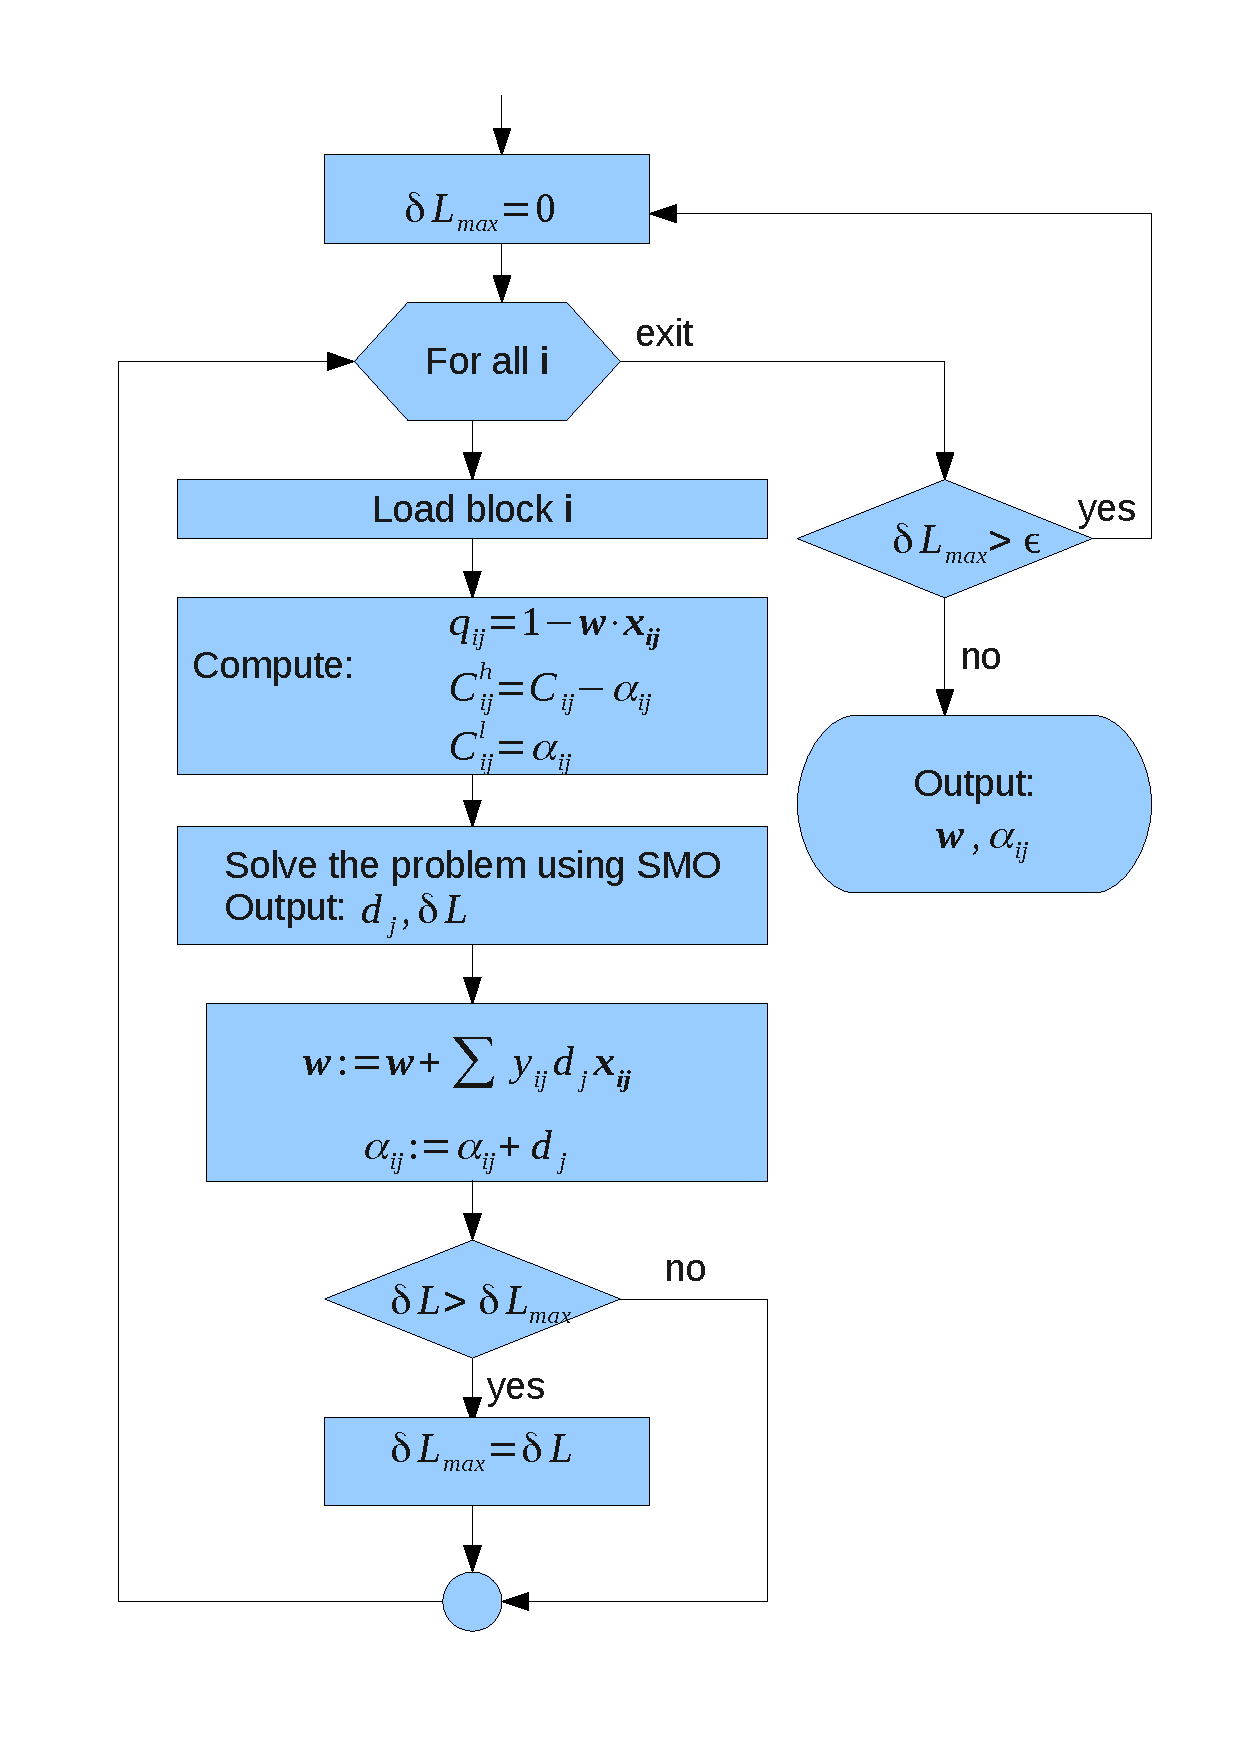
\includegraphics[scale=0.5]{Scoring/Fig/Algorithm.pdf}
\caption[The flowchart of block sequential minimal optimization algorithm]{
The flowchart of block sequential minimal optimization algorithm.
}
\end{center}
\label{Fig:flowchart}
\end{figure}

As it is seen from Eq. \ref{eq:eta}, our BSMO algorithm requires only scalar products of the structure vectors within the same block. Therefore, it is sufficient to 
load each block into RAM sequentially, which results in memory efficiency of our method. Precisely,  RAM required for our implementation of the block-decomposition solver 
is $N^2$ times less compared to the direct quadratic problem solvers. 

\subsection{Training database for protein-protein interactions}
\label{trainingSet}
In the present study we used the training database of 851 non-redundant protein-protein complex structures  prepared by Huang and Zou \cite{Huang2008}. 
This database contains  protein-protein complexes extracted from the PDB \cite{Berman2000} and includes 655 homodimers and 196 heterodimers. 
We updated three PDB structures from the original training database: 2Q33 supersedes 1N98, 2ZOY supersedes 1V7B, and 3KKJ supersedes 1YVV. 
The training database  contains only crystal dimeric structures determined by X-ray crystallography at resolution better than 2.5 \AA. 
Each chain of the dimeric structure has at least 10 amino acids, and the number of interacting residue pairs (as defined as having at least 1 heavy atom within 4.5 \AA) is at least 30. 
Each protein-protein interface consists only of 20 standard amino acids. 
No homologous complexes were included in the training database. 
Two protein complexes were regarded as homologues if the sequence identity between receptor-receptor pairs and between ligand-ligand pairs was $>70\%$. 
Finally, Huang and Zou \cite{Huang2008} manually inspected the training database and left only those structures that had no artifacts of crystallization. 

Our algorithm requires as input native and nonnative structure vectors (see, e.g., Eq. \ref{eq:planes}). Native structure vectors can be computed from the native 
protein-protein contacts in the training database using Eq. \ref{eq:projection}. 
However, for the computation of the nonnative structure vectors for each protein-protein complex from the training database, we need to generate decoys for each complex.
Since our optimization algorithm is very general and has no special requirements for nonnative protein-protein contacts, we generated them by "rolling" a 
smaller protein (ligand) over the surface of a bigger protein (receptor) using  HEX protein docking software \cite{Ritchie2000, hex}. 
To do so, we initialized HEX exhaustive search algorithm with the radial search step of 1.5 {\AA} and expansion order of the shape function equal to 31. We used only the 
shape complementarity energy function from HEX (i.e., electrostatic contribution was omitted). Afterwards, we clustered HEX docking results with a root mean square (RMS) 
threshold  of 8 {\AA}. The top 200 clusters, ranked by HEX surface complementarity function, plus the native protein-protein complex conformation 
(giving in total 201 structures) were then used to compute the distance distribution functions (Eq. \ref{eq:number_density}). 
Then, we computed the structure vectors using Eq. \ref{eq:projection} and labeled them as "native" if the root mean square deviation (RMSD) of the corresponding 
ligand was $<2$ {\AA} from its native position. Otherwise, the structure vector was labeled as "nonnative" or "decoy". 
On average, we obtained about 2.5 native structure vectors (and, correspondingly, about  198.5 nonnative structure vectors) per protein-protein complex.
To each structure vector $ \mathbf{x}_{ij}$ we assigned a regularization parameter $C_{ij}$ according to 
\begin{eqnarray}
\label{eq:regularizationParameter}
\begin{split}
C_{ij}^{native} = C{D_j^{nonnative}}/{D_j} \\
C_{ij}^{nonnative} = C{D_j^{native}}/{D_j}
\end{split}
\end{eqnarray}
%
We repeated the same procedure for each protein-protein complex from the training database.
We used $M=20$ atom-centered  interaction sites based on the atom types definitions provided by Huang and Zou \cite{Huang2008}. These atom types were defined by 
the classification of all heavy atoms in 20 standard amino acids according to their element symbol, aromaticity, hybridization, and polarity. 
These 20 atom types result in total of 210 pair potentials.
%For all the calculations in the presented study we used the cutoff value of 10 {\AA} . Accordingly, we chose the interval of orthogonality for 
%Legendre polynomials to be $[0;10]$. Convergence tolerance $\epsilon$ of the BSMO solver was set to $10^{-3}$.
%All computations were performed on a 32-bit Linux desktop computer with 4 Gb of RAM.

Our training set has several proteins homologous to the ones from the two widely used docking benchmarks, Rosetta, and Zdock, which we employ below to validate our results. 
We define two protein complexes to be homologous if for each chain in the first complex there is a chain in the second complex with sequence identity more than 60\%. 
We determined the sequence identity using the FASTA36 program \cite{Pearson1997}. Below, we benchmarked our scoring function while both excluding homologs from the training set
and leaving it unchanged. The comparison of the benchmark results in these two cases is shown in supplementary Tables S1 and S2.


%The training set has several homologs with the benchmarks we tested our functions on. We call two complexes homologous if for each chain in the first complex 
%there is a unique chain in the second complex with sequence identity is more than 60\%. The sequence identity was determined using FASTA36 program \cite{Pearson1997}.
%This criterion is different from the homology criterion during assembling of the training set.
%We benchmarked scoring functions using training set with and without corresponding homologs sets. %=======================================================================================================%


%WATER TRAINING DATABASE
\subsubsection{Training database for water-protein interactions}
To obtain potentials for the water molecules we employed the same set of complexes prepared by Huang and Zou \cite{Huang2008}. We added a new atom type to the set of 
20 atom types for docking corresponding to the water oxygen. We generated a cube with dimensions $130\times 130 \times 130\AA$ of TIP3P water molecules and equlibrated 
it using molecular dynamics at room temperature with periodic boundary conditions. Afterwards native structures and decoys from the training set were immersed into this water-box. In the case
when the size of the protein was more than $130\AA$ we periodically continued the water box. Then, in case of native structures initial water molecules presented in the 
crystallographic structures were retained. In the case of decoys we removed all the original water molecules. The placed bulk molecules were then removed if they clashed 
with either the proteins or retained water molecules. The clashing distance was set to be $2\AA$. We also removed each water molecules farther than $12\AA$ from all protein atoms.
Although we aimed to obtain all pairwise potentials we did not use water-water potential for the predictions, because it influences the equilibrium structure of bulk water,
thus in principle after obtaining this potential we had to recalculate water box. However this procedure goes beyond our method of obtaining scoring potentials.
